% -----------------------------------------------
% Template for ISMIR 2014
% (based on earlier ISMIR templates)
% -----------------------------------------------

\documentclass{article}
\usepackage{ismir2014,amsmath,cite}
\usepackage{graphicx}
\usepackage{url}
\usepackage{units}

% Title.
% ------
\title{Genre-specific Key Profiles}

% Single address
% To use with only one author or several with the same address
% ---------------
%\oneauthor
% {Names should be omitted for double-blind reviewing}
% {Affiliations should be omitted for double-blind reviewing}

% Two addresses
% --------------
%\twoauthors
%  {First author} {School \\ Department}
%  {Second author} {Company \\ Address}

% Three addresses
% --------------
\threeauthors
  {First author} {Affiliation1 \\ {\tt author1@ismir.edu}}
  {Second author} {\bf Retain these fake authors in\\\bf submission to preserve the formatting}
  {Third author} {Affiliation3 \\ {\tt author3@ismir.edu}}

% Four addresses
% --------------
%\fourauthors
%  {First author} {Affiliation1 \\ {\tt author1@ismir.edu}}
%  {Second author}{Affiliation2 \\ {\tt author2@ismir.edu}}
%  {Third author} {Affiliation3 \\ {\tt author3@ismir.edu}}
%  {Fourth author} {Affiliation4 \\ {\tt author4@ismir.edu}}

\begin{document}
%
\maketitle
%
\begin{abstract}
Pitch chroma are a popular feature for many MIR tasks. Using the GTZAN data set we investigate the distributions of pitch chroma for 9 different genres, the degree to
which these genres can be identified using these distributions and different strategies for achieving key-independence; namely transposition of the chroma according to its maximum value and 12-point FFT. We find that combining pitch chroma with commonly used MFCCs can lead to small increase in classification accuracy using a Support Vector Machine. Furthermore these results show that the imposing key-independence has a surprisingly small affect on performance.
\end{abstract}
%
\section{Introduction}\label{sec:introduction}
Musical genre recognition is a well studied field in MIR [*ref]. As with any classification task, the feature used to summarize tracks is an extremely important concern. Previous work in this area has shown that timbral features, particularly Mel Frequency Spectrum Coefficients, are especially suited to the task of predicting genre. While MFCCs are suited to picking up on instrumental and timbral difference between genres, some work has shown that they are not totally independent of harmonic or tonal information [*ref li]. Here we investigate the extent to which tonal information can be used to discern genres y examining the distributions of pitch chroma within each of 9 different genres. First we examine the overall distribution of keys for each genre. Next different methods for transposing pitch chroma to a key-independent representation are introduced and we look at the chroma distributions using chroma box plots, inter-genre distance and mulch-dimensional scaling. In the final section we test the degree to which the chroma distribution separate gen-res by performing classification with an SVM using chroma and combined chroma/MFCC features.

\section{Data set}\label{sec:dataset}
The data set used was the GTZAN collection, which is popular for genre classification tasks. It consists of a collection of $1000$ song excerpts divided into ten genres: Blues, Classical, Rock, Reggae, Pop, Metal, Rock, Jazz, Country and Hip Hop. First we examine the general layout of the data set, specifically with respect to the key distributions within genres. Key annotations for each track were produced manually and are publicly available.\footnote{\url{github.com/alexanderlerch/data_set}} Instances that included key modulations or where hard to identify have been omitted. The Classical genre has not been annotated. The number of annotated files reflects the difficulty of unambiguously identifying the key --- the number of annotated files is shown in the Table~\ref{tab:NumberOfAnnotatedDataSetEntries}. 

\begin{table}
    \begin{center}
        \begin{tabular}{|l|l|l|l|}
        \hline
        genre & \# major & \# min & \# annotated \\
        \hline
        blues 	&3 	    &95     &98\\
        \hline
        classic &0 	    &0 	    &0\\
        \hline
        country &94 	&5 	    &99\\
        \hline
        disco 	&43 	&55 	&98\\
        \hline
        hiphop 	&13 	&68 	&81\\
        \hline
        jazz 	&52 	&27 	&79\\
        \hline
        metal 	&4 	    &89 	&93\\
        \hline
        pop 	&44 	&50 	&94\\
        \hline
        reggae 	&53 	&44 	&97\\
        \hline
        rock 	&55 	&43 	&98\\
        \hline\hline
        overall &361    &476    &837\\
        \hline
        \end{tabular}
    \end{center}
   
	\caption{Number of annotated data set entries}
	\label{tab:NumberOfAnnotatedDataSetEntries}
\end{table}

Figure \ref{fig:KeyDistributionPerGenre} visualizes the distribution of keys for each genre.
\begin{figure}
    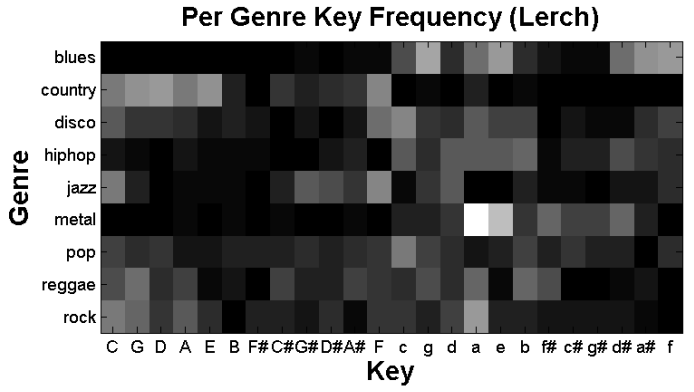
\includegraphics[scale=.4]{graph/key_distribution}
	\caption{Key distribution per genre (brighter means more frequent): SHIFT BOTH CMAJOR AND AMINOR TO THE MIDDLE}
	\label{fig:KeyDistributionPerGenre}
\end{figure}
The distribution of keys in each genre proved unsurprising.
The relation of major v.s.\ minor modes is very skewed for blues and metal (predominantly minor) as well as country (predominantly major), while the genres disco, pop, reggae, and rock appear to be quite balanced.
Jazz tracks tend to be clustered around flat keys which are favored by trumpet and saxophone players. 
The keys for country cluster around C-Maj with a tendency to sharp keys.
%Pieces from the blues are mostly in the keys of G, E and B-flat. 
The majority of metal tracks are in either a-min or e-min, keys that are well-suited to the electric guitar and bass and correspond to the two lowest open strings.


Li and Chan presented another set of key annotations for the GTZAN data set \cite{li_genre_2011}. An examination of the two independent annotations reveals some disagreements between the two annotations: overall, about $85$ percent of the data is labeled identically. Of the differences where there was disagreement on whether a key modulation occured or not, the majority were found in the Blues genre with 67 out 127 total disagreements of this type. If we consider only examples where both analyses agreed a modulation had \textit{not} occured, there was a total of 119 disagreements. The most common differences were: major/relative-minor confusion (38), root/fifth confusion (35) and major/minor confusion (13).
DISCUSS DIFFERENCES MORE IN DETAIL??
%\begin{itemize}
    %\item   blues: $98$ vs.\ $31$ (Li) annotated tracks
    %\item   disco: $21$ differences between the two data sets
%\end{itemize}
%The genre country showed only $1$ difference. 

\section{Feature extraction}\label{sec:pitch_chroma}
We extract the key profiles per file. The term key profile as we use it here is the overall, root-note independent pitch chroma per file. The detailed extraction is explained below.

\subsection{Pitch chroma}\label{subsec:pc_extract}
The pitch chroma is a commonly used feature in the field of Music Information Retrieval (MIR) \cite{muller_information_2007}. It is a twelve-dimensional histogram-like octave-independent vector showing the “strength” of the 12 semitone classes (C, C\#, D, ..., B). It is computed by converting the spectrum to semi-tone bands and summing the energy of all bands with the distance of an octave \cite{fujishima_realtime_1999}. The overall pitch chroma per file is a single 12-dimensional vector that is computed by taking the median of all individual pitch chromas. 
The pitch chroma is extracted at a sample rate of \unit[10]{kHz} over a range of three octaves, starting from C at \unit[130.8]{Hz}. The FFT block size is XXX, the hop size is XXX.

 %Each track in the labeled collection was down-sampled to 10kHz and pitch chroma vectors were extracted block-wise over a three octave range, starting from C = 130.8 Hz. Pitch chroma were then normalized using the 1-norm:                     
	 %equation?
%After extracting pitch chroma for each block we can also average them over whole tracks to obtain an “averaged pitch chroma” for each track, sometimes called a Pitch Histogram [**ref]. After averaging using the median for each chroma-bin each song is then represented by a single 12-dimensional chroma vector.


\subsection{Key profile}
We assume that the pitch chroma of a song in the same mode (major or minor) should be similar between songs within one genre, but is shifted circularly to the song's root note. Under this assumption, we can ``convert'' each pitch to a key-profile by applying a circular shift to make it root-note independent. In other words, the key profile is the root note independent pitch distribution (e.g., the pitch profile of a song in A-Maj or a-min is circularly shifted by nine indices to the left so that the bin of pitch class A lands on the first index).

%A problem with using a pitch chroma approach is that the overall tonality of each song may dominate any between-genre differences; because the distribution of major and minor keys are not the same for each genre, songs might be classified according to their key using this method. For example pitch chroma extracted from minor tracks would be classified as Metal, since the averaged pitch chroma for Metal would be obtained by averaging pitch chroma extracted from predominantly minor tracks. This is an inherent problem in using pitch chroma as op-posed to more often used timbral features like MFCCs and in order to account for this we processed major and minor tracks separately. Another consideration revealed in the analysis of the data set is that the the key-labels are not uniformly distributed within each key. For example the majority of songs in the keys of A and E-minor are in the Rock and Metal genres. 

We investigated the following approaches to obtaining a key-independent representation.

\subsubsection{Transposition by ground truth}
The overall pitch chroma of each song is shifted by the root note index annotated in the ground truth.

\subsubsection{Transposition by max}
The overall pitch chroma of each song is shifted by the index of the maximum of this pitch chroma. This can be interpreted as the simplest possible root note estimation.

\subsubsection{Fourier transform}
The shift dependent on the root note can be understood as the phase of the pitch chroma. The magnitude spectrum of the extracted pitch chroma is thus a phase-independent (and therefore root-note independent) representation.
%Firstly, for a given pitch chroma vector the mean over all bins is calculated and is subtracted from each component. 

\section{Results}
\subsection{Overall key profiles}
Figure \ref{fig:OverallKeyProfiles} shows the overall key profiles in a box plot in comparison with two widely-used measures. Krumhansl's ``Probe Tone Ratings'' \cite{krumhansl_cognitive_1990} are not really a key profile, but has been frequently used in audio key detection since they seem to correlate well (e.g., \cite{izmirli_template_2005}). Temperley's key profiles \cite{temperley_tonal_2007} are derived from symbolic data rather than from audio. MAKE SURE THE TEMPERLEY PROFILES ARE THE SAME AS IN THE IZMIRLI PAPER AND THIS IS THE CORRECT CITATION (DONT HAVE THE BOOK).
\begin{figure*}[tb]
    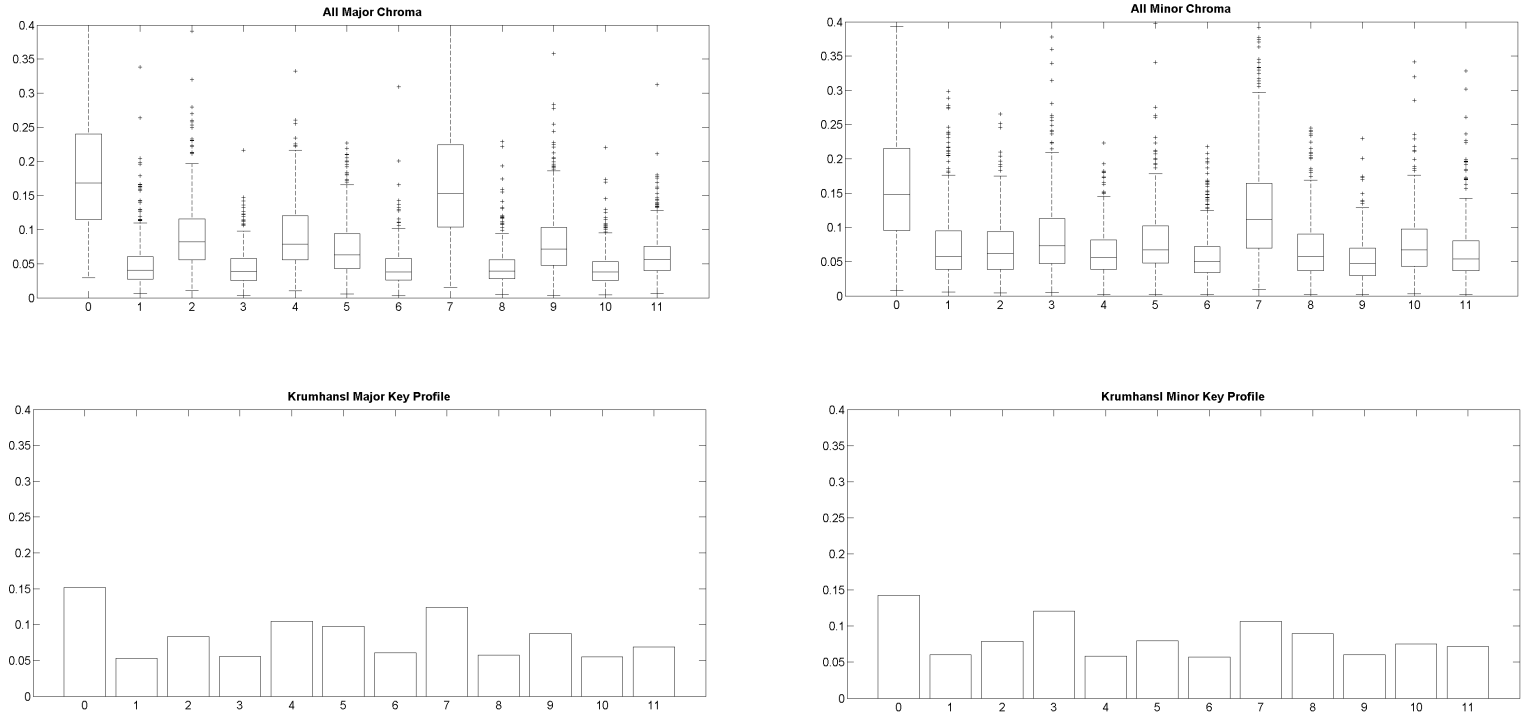
\includegraphics[scale=.4]{graph/overall_boxplot}
	\caption{Major (left) and minor (right) key profiles for the complete data set, in comparison with two widely-used key profiles (Krumhansl and Temperley) CAN YOU OVERLAY THE BOX PLOTS WITH THE KRUMHANSL/TEMPERLEY GRAPHS? SHOULDNT THE WHISKERS BE THERE FOR ALL PITCHES?}
	\label{fig:OverallKeyProfiles}
\end{figure*}

\subsection{Genre-specific key profiles}
The key profiles of the six most populated genres is plotted in Fig.~\ref{SpecificKeyProfiles}.
\begin{figure*}[tb]
    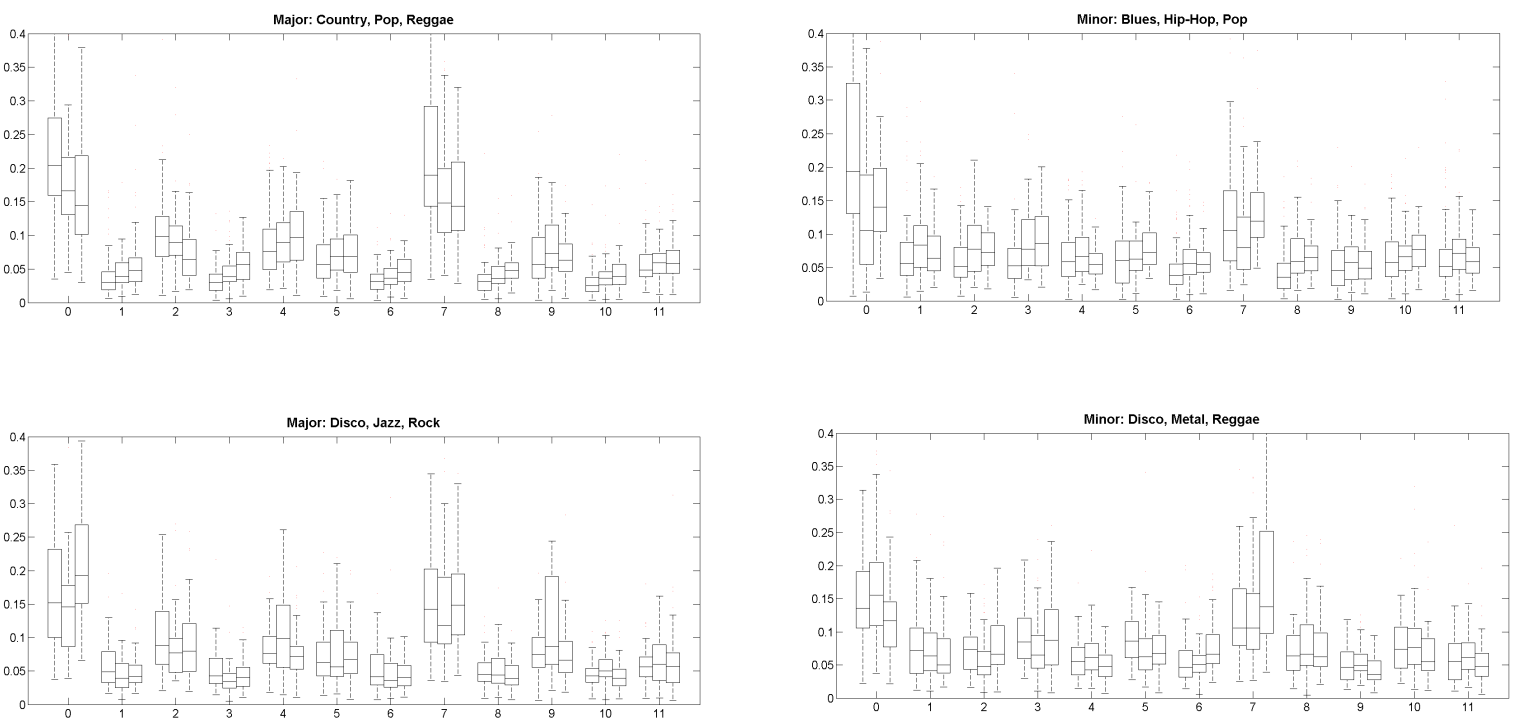
\includegraphics[scale=.4]{graph/specific_boxplot}
	\caption{Major (left) and minor (right) key profiles for the various genres, in comparison with two widely-used key profiles (Krumhansl and Temperley) CAN YOU OVERLAY THE BOX PLOTS WITH THE KRUMHANSL/TEMPERLEY GRAPHS? SHOULDNT THE WHISKERS BE THERE FOR ALL PITCHES?}
	\label{fig:SpecificKeyProfiles}
\end{figure*}

\subsection{Inter-genre distances}
In order to evaluate how distinct genres are with respect to their key profile, distance between all profiles were calculated using the Manhattan distance as shown in Figs.~\ref{fig:distance_major} and \ref{fig:distance_minor}. Genres for which the number of examples were less than 30 are grayed out. The labels are as follows: B is blues, C country, D disco, H hip-hop, J jazz, M metal, P pop, Rg Reggae, Rk is rock, K is the Krumhansl key profile and T the Temperley profile \cite{temperley_tonal_2007}.
\begin{figure}[tb]
    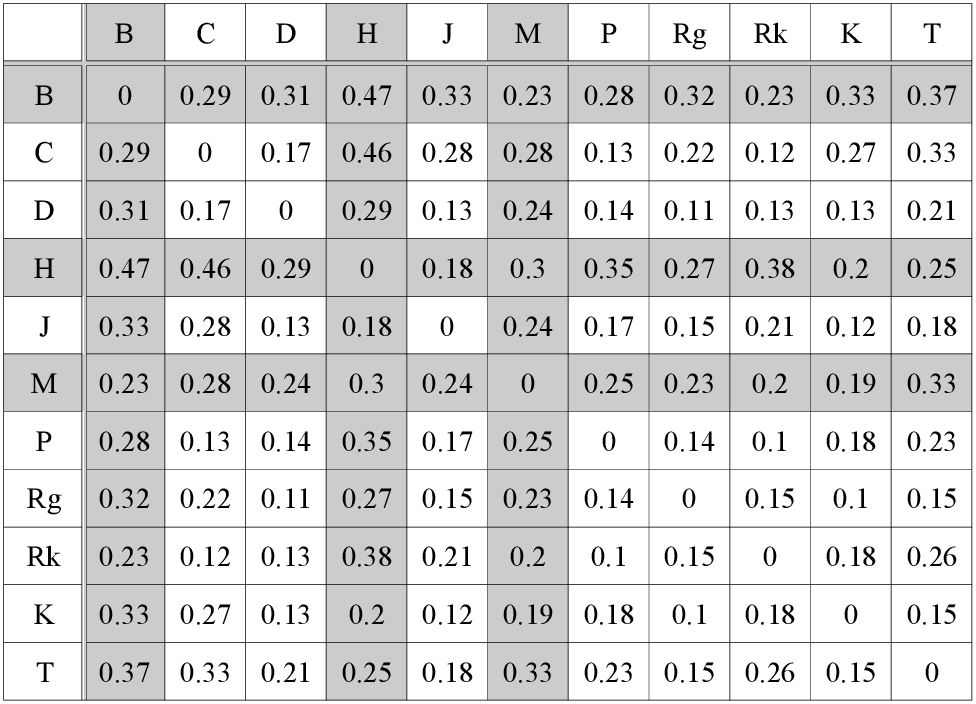
\includegraphics[scale=.4]{graph/majorDistManhattan}
	\caption{Manhattan distance between the major profiles of all genres and three overall profiles MAYBE INCLUDE THE OVERALL MEDIAN VALUES HERE AS WELL}
	\label{fig:distance_major}
\end{figure}
\begin{figure}[tb]
    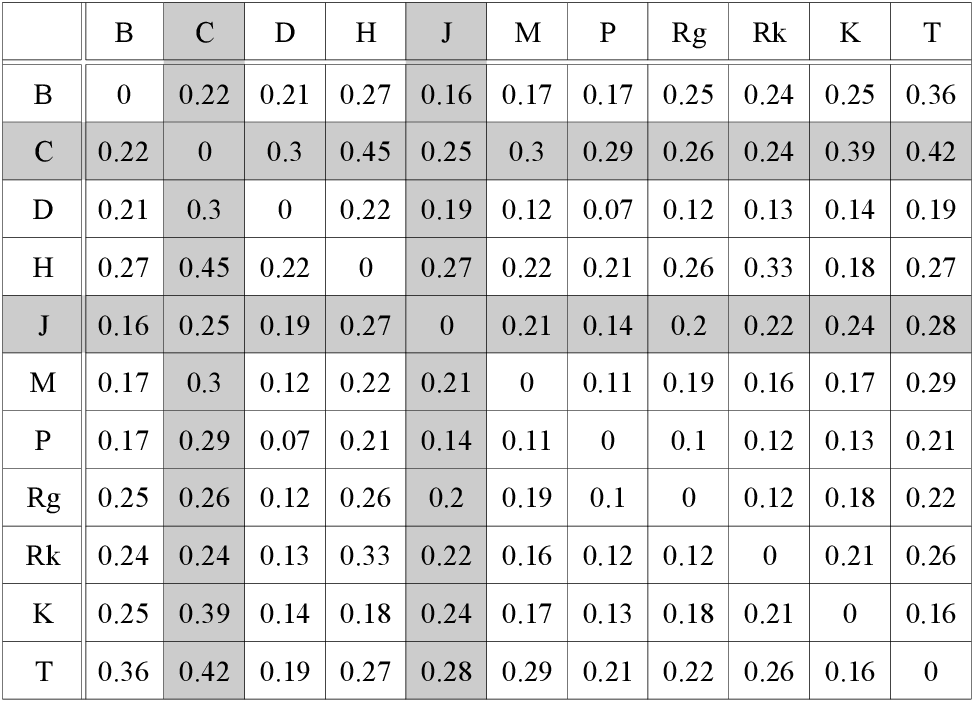
\includegraphics[scale=.4]{graph/minorDistManhattan}
	\caption{Manhattan distance between the minor profiles of  all genres and three overall profiles MAYBE INCLUDE THE OVERALL MEDIAN VALUES HERE AS WELL}
	\label{fig:distance_minor}
\end{figure}


\subsection{Discussion}
Overall each genre roughly exhibits the expected major pattern with some exceptions, for example,  Jazz. The Jazz distribution is noticeably more flat than other genres --- it doesn't exhibit the same peakiness at the root and fifth for example and the relative ratios of each interval are noticeably more uniform. This agrees with the classification results of Section 5, where Jazz was one of the least confused major genres.

For the minor examples, the distributions look much more uniform with relatively more mass in non-diatonic bins --- for example the flat-second (C\#) and-sharp fifth (G\#) genres.

Some facts revealed from the key profile distances, the most mutually distinct genres when considering major tracks are Country and Jazz while the the most similar are Rock and Pop. For minor tracks, Reggae and Pop are most similar while Reggae and Rock are the most distinct.


\section{Classification}
While the distance results indicate what genres are most similar and dissimilar, it does not allow an interpretation as to whether the genres distances do actually help to separate genres. To investigate this effect, we train and evaluate a Support Vector Machine using libSVM \cite{chang_libsvm:_2011}.
The SVM hyper-parameters (C, γ) representing the margin and kernel widths were tuned using a grid-search and 5-fold cross validation on a separate stratified split of the data (I HAVE NO IDEA WHAT THAT MEANS). Best performance was achieved using a non-linear SVM with Radial Basis Function kernel.
We investigated the following scenarios: (i) the whole key-labeled data set with no differentiation between major and minor and (ii) the major/minor subsets individually in order to control for the differences in major/minor distribution between keys. 
10-fold cross validation  accuracy was calculated using the raw pitch chroma, max-shifted key profile, the Fourier pitch chroma and the key profile shifted according to the ground truth. We compare the results to a classifier based on a set of MFCC features as well as a combination of MFCC and key profile features. MFCC features were calculated according to REFXXX: WHAT COMPUTATION DID YOU USE?. The mean and standard deviation of $12$ MFCCs form a $24$-dimensional timbre feature vector. %as follows: for each block we compute 12 MFCC coefficients, then take the mean and standard deviation over the whole song. These features are then concatenated to form a 24 dimensional feature vector.

Table~\ref{tab:accuracyPC} summarizes the results of the SVM classification for the different key profile computations, and Tab.~\ref{tab:accuracyPC+MFCC} shows the mode-independent results when combined with the MFCC features.
\begin{table}[tb]
    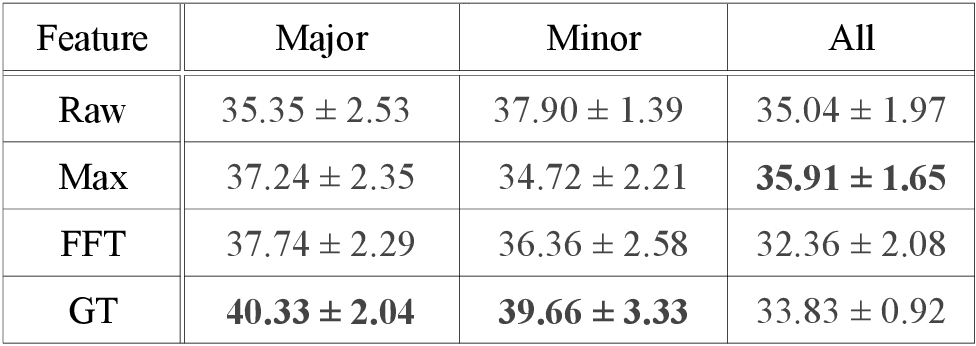
\includegraphics[scale=.4]{graph/accuracyPC}
	\caption{Classification accuracy for different key profile computations}
	\label{tab:accuracyPC}
\end{table}
\begin{table}[tb]
    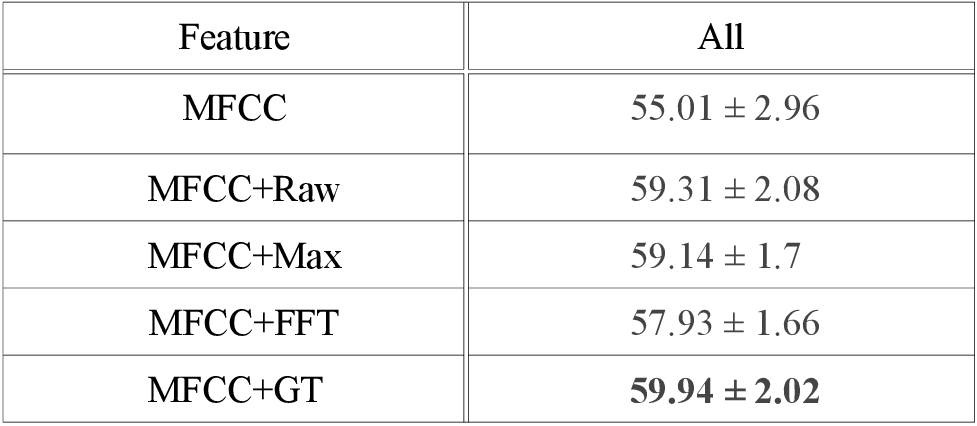
\includegraphics[scale=.4]{graph/accuracyPC+MFCC}
	\caption{Classification accuracy for different key profile computations in combination with MFCC features}
	\label{tab:accuracyPC+MFCC}
\end{table}
%MAYBE INCLUDE A 'BASELINE' CLASSIFICATION BASED ONLY ON THE KEY (NOT THE PITCH CHROMA) HERE FOR COMPARISON???

Figures \ref{fig:confMatMajPC}, \ref{fig:confMatMinPC}, and \ref{fig:confPC+MFCC} display the confusion matrices of the classification results. PLEASE ADD ANOTHER ROW TO THE MATRICES WITH THE SUM OVER ROWS - BUT WE HAVE TO REDO ALL OF THESE ANYWAY, WE DONT WANT THEM AS PNGs.
\begin{figure}[tb]
    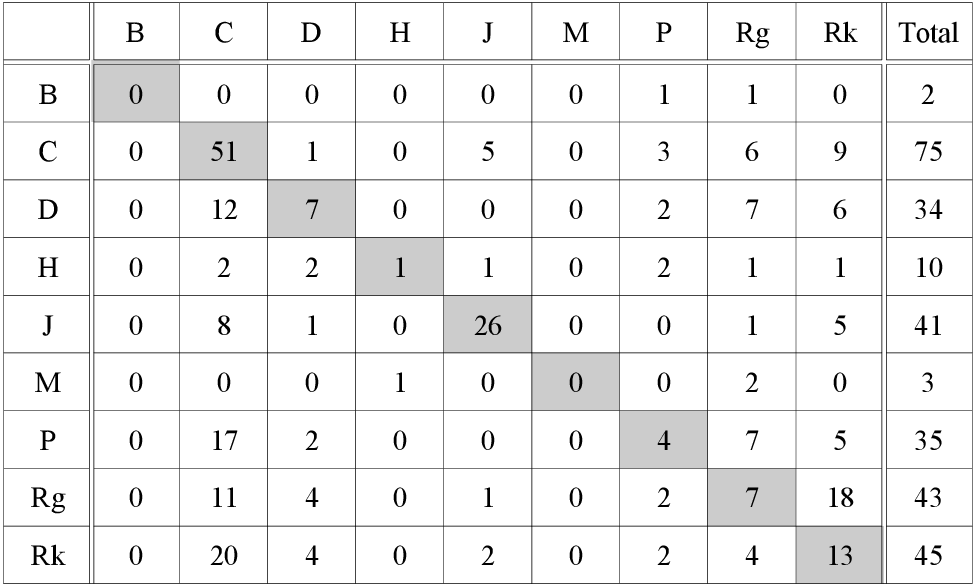
\includegraphics[scale=.4]{graph/confMatMajPC}
	\caption{CONFUSION MATRIX 1, major}
	\label{fig:confMatMajPC}
\end{figure}
\begin{figure}[tb]
    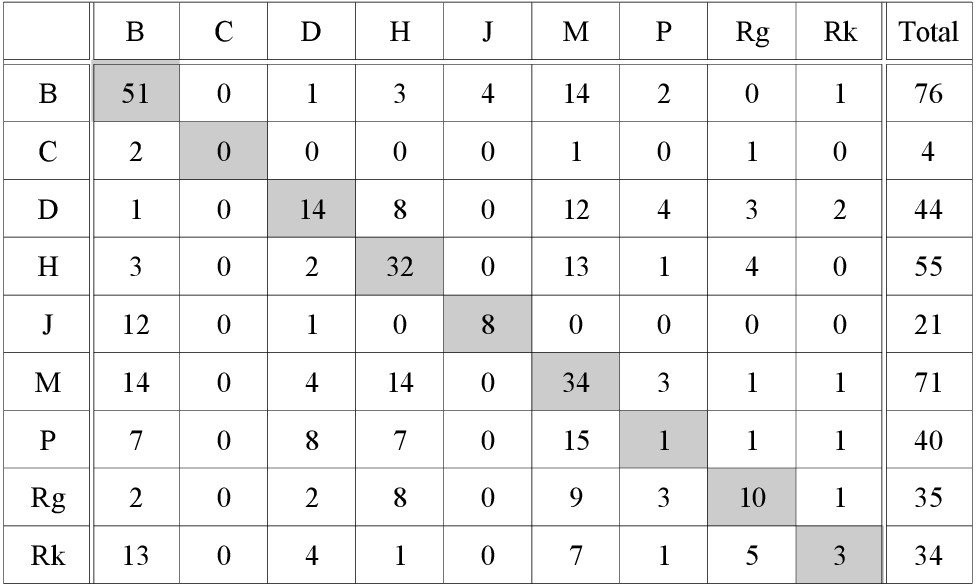
\includegraphics[scale=.4]{graph/confMatMinPC}
	\caption{CONFUSION MATRIX 2, minor}
	\label{fig:confMatMinPC}
\end{figure}
\begin{figure}[tb]
    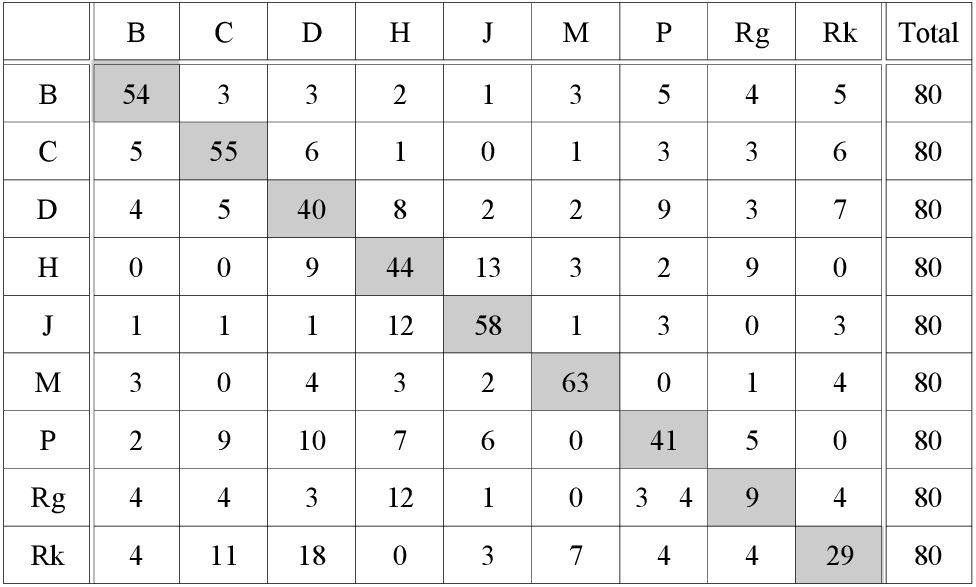
\includegraphics[scale=.4]{graph/confPC+MFCC}
	\caption{CONFUSION MATRIX 3, pc + mfcc}
	\label{fig:confPC+MFCC}
\end{figure}
DESCRIBE AND DISCUSS ME.

\subsection{Results and discussion}
One fact revealed in this analysis is the relatively small performance increase observed by sorting the chroma, even when using the ground truth directly. By sorting the chroma any information on the genre given by the key has been removed (for example as a prior estimate based on the key distributions in each genre) which would, it is hoped, reveal any differences in the distributions. 
However, whether or not this technique improves performance depends on the initial distribution of pitch chroma; suppose genre groups are perfectly separable given their key-independent chroma distributions and then for each song we transpose it into a new key with some related probability. Since cyclic-transpositions correspond to reflections this process is unlikely to make the data significantly more or less separable, which may explain the small in-crease in performance when using sorted chroma. I STILL CANNOT FOLLOW HERE!
Splitting the data into major and minor results in slightly improved accuracy, however in this case we have added information by using the ground truth and realistically harmony estimation should be done automatically which would be an additional source of error.
	Unsurprisingly MFCCs vastly outperformed pitch chroma features alone. However, combining features results in a slight performance increase in overall accuracy of around 4-5% indicating that the pitch chro-ma distributions contain at least some genre-relevant information.
    
    MENTION RANDOM CLASSIFICATION RATE - SHOULD BE AROUND 11\%, but we have nonuniform class distributions.
    
    LETS NOT FORGET THAT WE DO NOT ACTUALLY WANT TO CLASSIFY, WE JUST WANT TO SHOW THAT THE GENRES ARE SEPARABLE WRT THEIR KEY PROFILE.
    
    DISCUSS CONFUSION MATRICES

\section{Conclusion}
\begin{itemize}
    \item   some genres are separable, but overall the similarities between the key profiles outweigh the differences
    \item   mention most similar and most separate genres
    \item   not a proposal to use these profiles but to investigate whether there are genre dependent differences or not.
\end{itemize}


\bibliography{ChromaPaper}

\end{document}
